\section{La categoría AutoModelCar}

\begin{frame}\frametitle{La categoría AutoModelCar}
  \begin{itemize}
  \item Se originó por el proyecto \textit{Visiones de movilidad urbana} a través del cual se donaron vehículos a escala a varias instituciones educativas y de investigación del país
    \begin{figure}
      \centering
      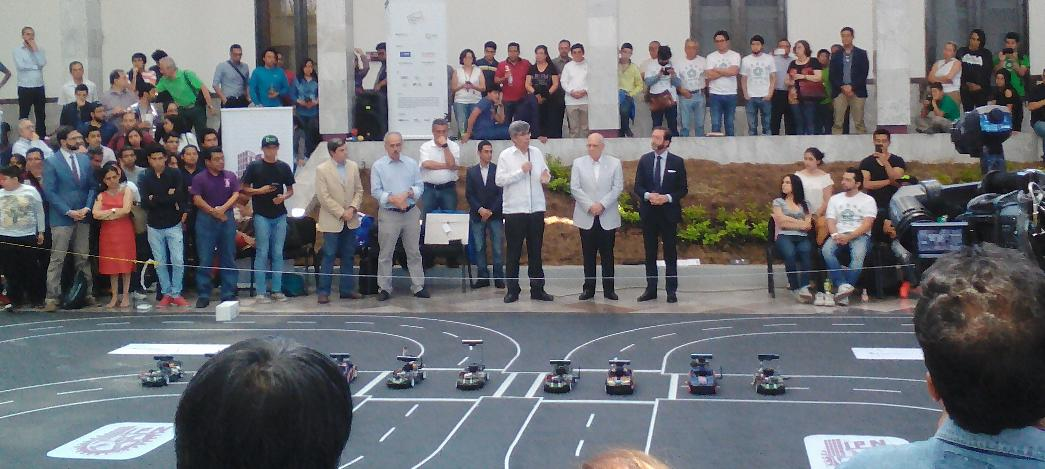
\includegraphics[width=0.9\textwidth]{Figuras/VisionesDeMovilidadUrbana.jpg}
    \end{figure}
  \end{itemize}
\end{frame}

\begin{frame}\frametitle{La categoría AutoModelCar}
  \begin{itemize}
  \item Originalmente solo se permitían vehículos AutoNOMOS:
    \begin{figure}
      \centering
      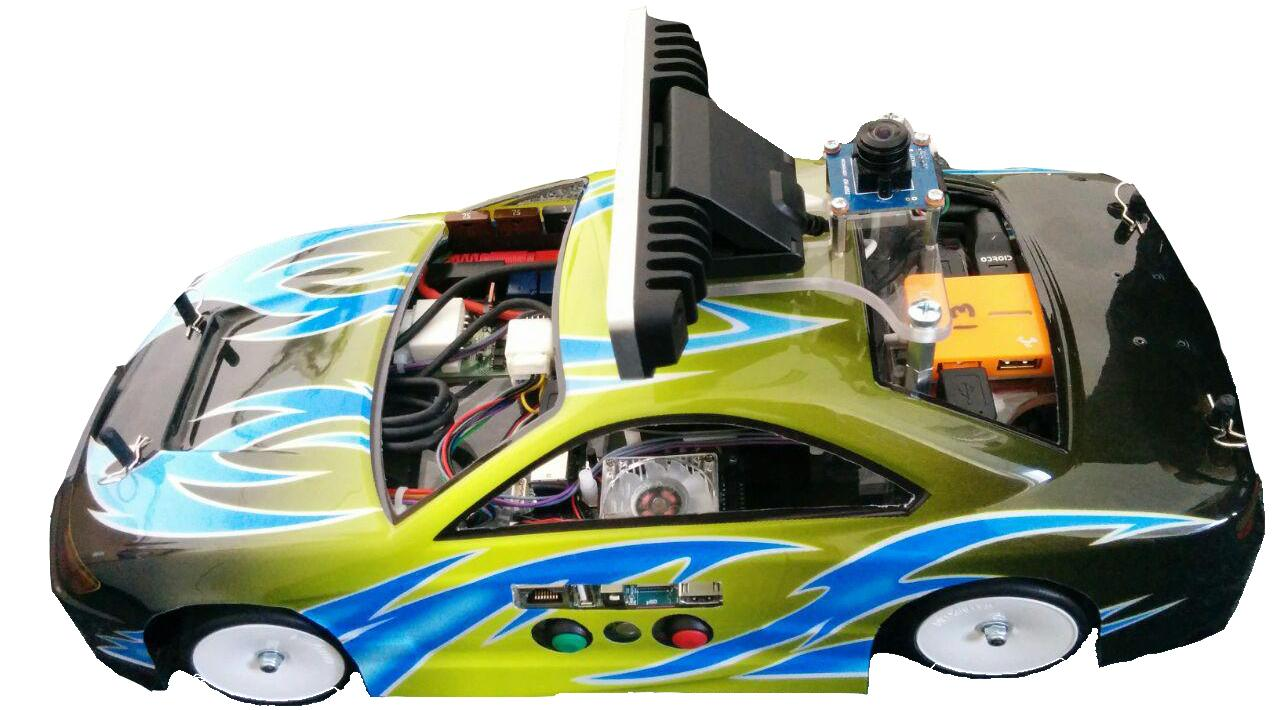
\includegraphics[width=0.35\textwidth]{Figuras/AutoNOMOS.jpg}
    \end{figure}
  \item Pero ahora se puede participar con cualquier vehículo a escala:
    \begin{figure}
      \centering
      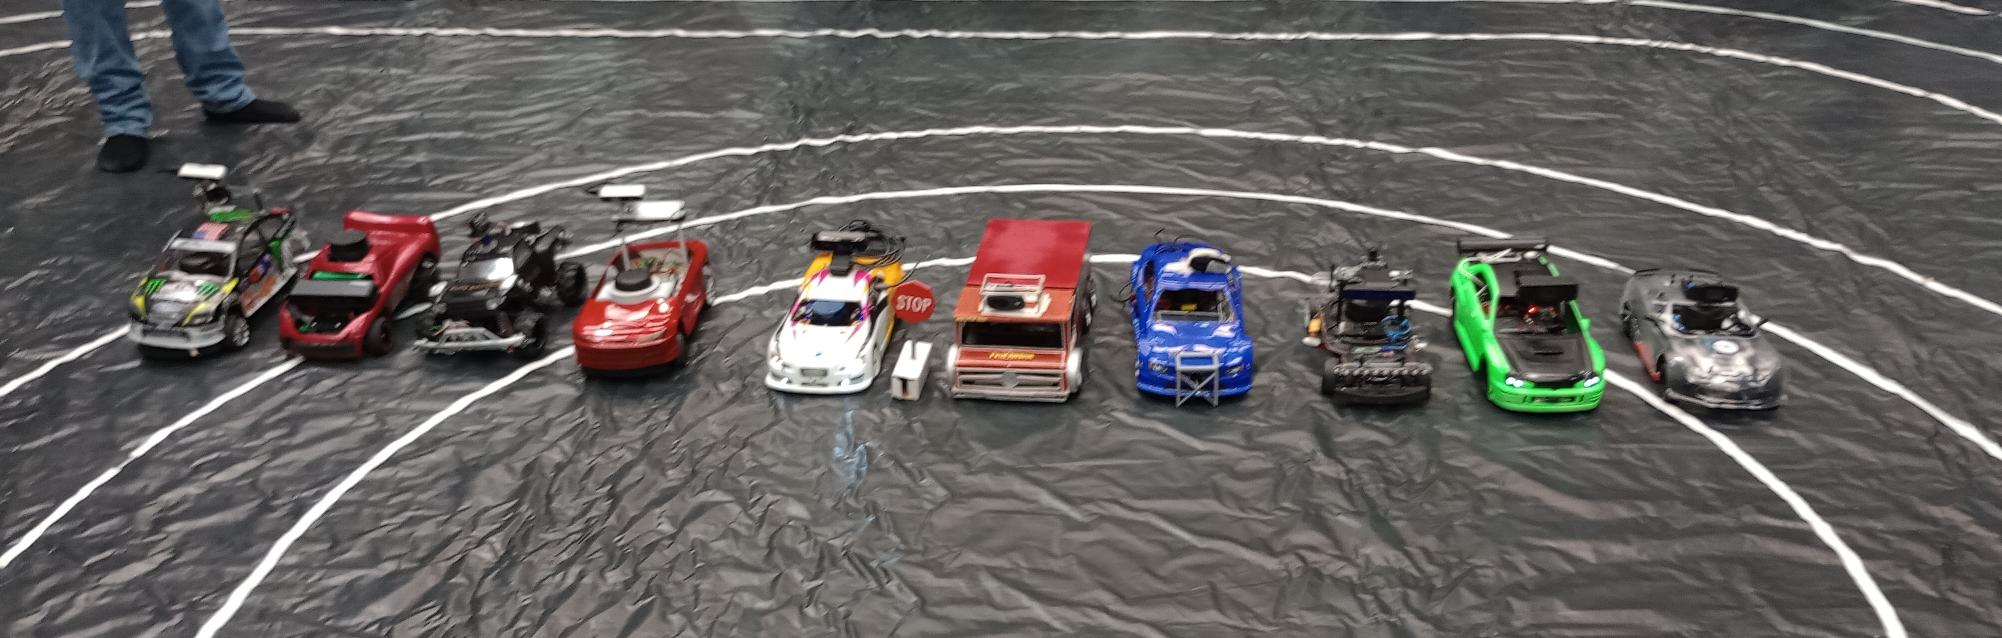
\includegraphics[width=0.75\textwidth]{Figuras/AutoModelCarCars.jpg}
    \end{figure}
  \end{itemize}
\end{frame}

\begin{frame}\frametitle{La categoría AutoModelCar}
  \begin{itemize}
  \item La competencia consta de cuatro pruebas (esperemos aumentarlas este año):
    \begin{multicols}{2}
      \begin{itemize}
      \item Navegación autónoma sin obstáculos
      \item Navegación con obstáculos estáticos
      \item Navegación con obstáculos en movimiento
      \item Estacionamiento
      \end{itemize}
    \end{multicols}
    \begin{figure}
      \centering
      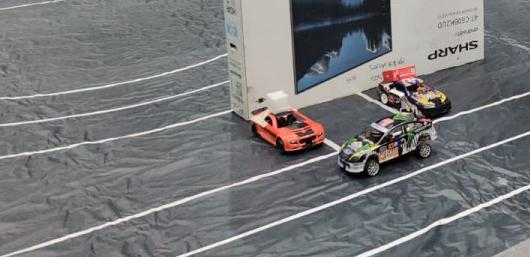
\includegraphics[width=0.6\textwidth]{Figuras/AutoModelCarEstacionamiento.jpg}
    \end{figure}
  \end{itemize}
\end{frame}

\begin{frame}\frametitle{La categoría AutoModelCar}
  Se utiliza una pista con rectas, curvas y cruces:
  \begin{figure}
    \centering
    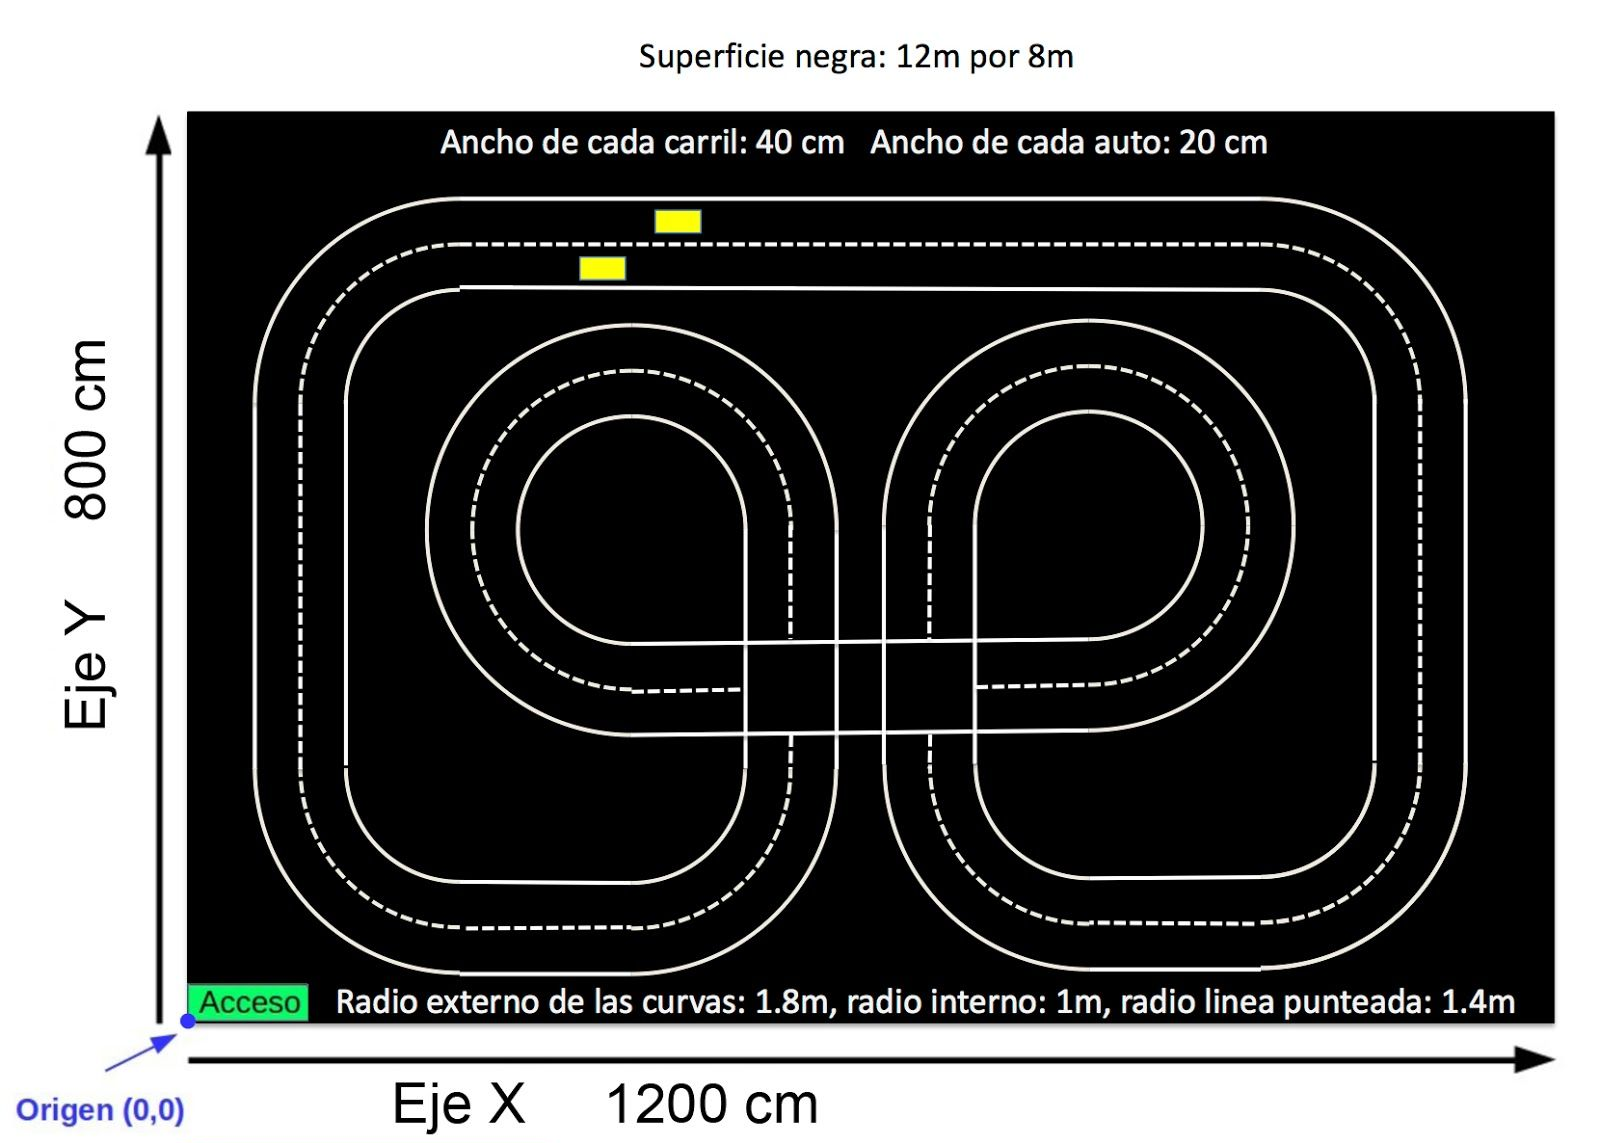
\includegraphics[width=0.7\textwidth]{Figuras/AutoModelCarPista.png}
  \end{figure}
\end{frame}

\begin{frame}\frametitle{Hardware para vehículos sin conductor}
  \begin{figure}
    \centering
    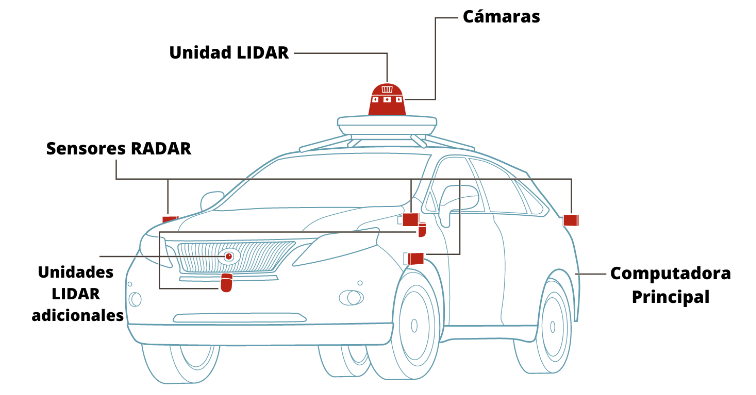
\includegraphics[width=0.6\textwidth]{Figuras/Hardware.png}
  \end{figure}
\end{frame}

\begin{frame}\frametitle{El simulador Webots}
  
\end{frame}